\section{Related Work}
\label{app:related_work}

\subsection{Generative VLA Models}
Embodied intelligence is shifting from task-specific policies toward unified Vision-Language-Action (VLA) foundation models. Representative works have shown that combining large-scale vision-language pretraining with robot control can substantially improve cross-task generalization, semantic understanding, and cross-platform transfer \cite{o2024open,black2024pi_0,zitkovich2023rt,kim2024openvla,ghosh2024octo,li2023vision,bjorck2025gr00t,pertsch2025fast,song2025accelerating}. On the action modeling side, modern VLA and general robot policies often adopt generative frameworks to model high-dimensional, continuous, and multi-modal action distributions: diffusion models generate actions through iterative denoising \cite{chi2025diffusion,wen2025diffusionvla,black2024pi_0,chen2025fast,li2025cogvla,zhao2025cot,hou2025dita,kim2025fine,song2025hume}, while flow matching directly learns velocity fields along continuous trajectories. These approaches typically offer stronger action expressivity, but they also incur higher policy-call cost\cite{wang2024one}. Consequently, reducing control latency without sacrificing generation quality has become a central challenge in deploying VLA models.

\subsection{Action Chunk and Horizon Trade-off}
To alleviate the tension between high-frequency control and expensive policy inference, \textbf{action chunk} has been widely adopted in continuous control. The core idea is to predict multiple future actions in a single inference call and then execute them sequentially with a downstream controller \cite{chi2025diffusion,zhao2023act,black2024pi_0,shukor2025smolvla,bjorck2025gr00t,wang2025sigma,driess2025knowledge}. This design effectively amortizes policy-call frequency and improves temporal smoothness, but it also reduces the use of fresh observations within a fixed action horizon. A longer horizon further lowers inference frequency and maintains action consistency, but weakens responsiveness to environmental changes; a shorter horizon more closely resembles strict closed-loop control and often provides better local recovery, yet requires much more frequent policy calls \cite{jing2025mixture,zhangaction,liu2024bidirectional,khan2025test,so2025improving,fu2025deep,zhao2026action,liu2026long}. Most existing approaches therefore seek a compromise under a static horizon, whereas our work focuses on an event-triggered dynamic horizon: the system retains the efficiency of long chunks during stable phases and truncates them on demand to recover closed-loop responsiveness during local failures.

\subsection{Failure Recovery in Visuomotor Policies}
Long-horizon visuomotor control commonly suffers from compounding errors and covariate shift: once execution drifts away from the training distribution, the policy often cannot recover on its own. Existing approaches can be broadly divided into two categories. One line of work expands the training distribution through additional interaction, human intervention, or recovery data collection, and then updates the policy accordingly \cite{sharma2023self,ingelhag2025real,hu2025rac,neary2025improving}. Another line explicitly introduces recovery policies, search mechanisms, or distributional constraints to pull the system back to a safe region once it departs from the expert manifold \cite{gao2025out,sun2025latent,jain2025smooth,liang2026adaptive,gou2024learning,wu2026speedup,xuvla}. These works collectively show that explicit recovery mechanisms can substantially improve the robustness of visuomotor policies; however, they typically rely on additional recovery data, separately trained recovery modules, or joint optimization tailored to a specific policy backbone.


% ============================================================
\section{Method Details}
\label{app:method_details}

\subsection{Details of Event-Triggered Truncation}
\label{app:event_trigger_details}

This section provides the full event-triggered truncation rule used by LVM. Given the online inconsistency score $E_t$, the monitor maintains a sliding window of recent scores,
\[
\mathbf{E}_W=\{E_{t-w+1},\dots,E_t\}.
\]
Let
\[
M_e=\mathrm{median}(\mathbf{E}_W),
\qquad
\mathrm{MAD}=\mathrm{median}\!\left(|E_i-M_e|\right),\quad E_i\in\mathbf{E}_W .
\]
We use the median absolute deviation because it is less sensitive to transient score spikes than the mean and variance. Based on this robust statistic, we define asymmetric on/off thresholds,
\[
T_{\mathrm{on}}=M_e+\lambda_{\mathrm{on}}\mathrm{MAD},
\qquad
T_{\mathrm{off}}=M_e+\lambda_{\mathrm{off}}\mathrm{MAD},
\qquad
\lambda_{\mathrm{on}}>\lambda_{\mathrm{off}}.
\]
The higher threshold $T_{\mathrm{on}}$ is used to confirm abnormal deviation, while the lower threshold $T_{\mathrm{off}}$ provides hysteresis and prevents rapid oscillation between normal and abnormal states.

To avoid triggering on isolated spikes, we maintain a persistence counter:
\begin{equation}
c_t =
\begin{cases}
c_{t-1}+1, & \text{if } E_t>T_{\mathrm{on}},\\
0, & \text{if } E_t<T_{\mathrm{off}},\\
c_{t-1}, & \text{otherwise}.
\end{cases}
\label{eq:debounce_counter_app}
\end{equation}
An interrupt event is triggered when
\begin{equation}
c_t\ge p,
\label{eq:meltdown_trigger_app}
\end{equation}
where $p$ is the patience parameter. After an interrupt event, the remaining actions in the current execution queue are discarded, the counter is reset, and the next policy query is performed under corrective mode. If $h$ actions have already been executed from the current queue, the realized action horizon is
\[
H_{\mathrm{adaptive}}=h<H.
\]
In this way, the system preserves long-horizon execution during stable phases, while shortening the horizon when persistent visual drift indicates that the current action chunk is no longer reliable.

\subsection{LVM and OGG Runtime Parameters}
\label{app:runtime_parameters}

\textbf{LVM monitoring parameters.}
The Latent-space Vision Monitor uses a robust online thresholding state machine. We maintain a sliding window of recent inconsistency scores with window size 15. The dynamic thresholds are computed using $\lambda_{\mathrm{on}}=3.0$ and $\lambda_{\mathrm{off}}=2.0$. An interrupt event is triggered only when the inconsistency score exceeds the activation threshold for $p=5$ consecutive steps. Similarly, the monitor requires 5 consecutive safe steps for reset. To avoid repeated triggers immediately after intervention, we use an interrupt cooldown of 10 steps.

\textbf{OGG parameters.}
Online Gradient Guidance is invoked only for the single policy query immediately following an interrupt-triggered truncation. When an interrupt event occurs, the remaining action queue is cleared, the next replan is marked as a guidance replan, and OGG is applied during that next action-chunk generation. Subsequent policy calls return to standard inference unless another interrupt event is detected. The guidance strength is controlled by $\eta$. In our experiments, we use $\eta=1$ as the default setting for $\pi_{0.5}$, SmolVLA, and X-VLA. The sensitivity of performance to $\eta$ is analyzed in Table~\ref{tab:eta_ablation}.

% ============================================================
\section{Training and Implementation Details}
\label{app:implementation_details}

\subsection{Benchmarks and Evaluation Protocol}
\label{app:benchmark_protocol}

We evaluate VLA-Corrector on two simulation benchmarks: MetaWorld~\cite{yu2020meta} and LIBERO~\cite{liu2023libero}. MetaWorld tests contact-rich manipulation robustness across difficulty splits, while LIBERO evaluates language-conditioned long-horizon task execution. We use $\pi_{0.5}$~\cite{intelligence2025pi_} as the main backbone, and further test SmolVLA~\cite{shukor2025smolvla} and X-VLA~\cite{zheng2025x} for cross-architecture evaluation. We report task success rate as the primary metric, together with policy calls, success-per-call efficiency, and post-interrupt recovery rate when applicable.

For MetaWorld, tasks are grouped into four difficulty splits: \emph{Easy}, \emph{Medium}, \emph{Hard}, and \emph{Very Hard}. All online evaluations are conducted task by task within each split, and we report the average success rate over tasks in the corresponding split. Unless otherwise specified, each task is evaluated with 20 episodes. For the corrector data-scaling study, we use a fixed episode-level split before subsampling the training data: 10\% of episodes are held out for validation, 10\% are held out for testing, and the remaining episodes form the training pool. We then subsample this training pool according to the training ratio $r$. In the multi-seed data-scaling analysis, we use split seeds $\{42,123,999\}$ and require at least 20 episodes in the train, validation, and test partitions. All simulation experiments are conducted on 8 NVIDIA A100-SXM4-40GB GPUs.

\subsection{External Corrector Architecture}
\label{app:corrector_architecture}

The external corrector $M_\phi$ is implemented as a residual MLP for short-horizon latent dynamics prediction. We first map the executed action through a linear embedding layer, concatenate the resulting action feature with the current visual latent $Z_t^{\mathrm{real}}$, and feed the combined representation into a stack of residual MLP blocks. The network predicts the short-horizon latent residual rather than the absolute future latent state. In all experiments, we use a four-layer hidden configuration with width $[2048,2048,2048,2048]$. The exact number of parameters varies slightly across benchmarks and VLA backbones because both the action dimensionality and the visual latent dimensionality differ across settings. Overall, the correctors used in our experiments contain approximately 38--42M parameters, and we refer to this external module as a lightweight $\sim$40M MLP corrector.

\subsection{Corrector Training}
\label{app:corrector_training}

The corrector is trained after the VLA backbone has been fine-tuned on the benchmark training set. We freeze the VLA backbone and use its visual encoder to extract latent representations from demonstration trajectories. The corrector is then trained on these frozen latents to predict the short-horizon visual latent residual induced by the executed action. We use AdamW as the optimizer with learning rate $3\times10^{-4}$ and weight decay $10^{-4}$. The learning rate is scheduled by cosine annealing with $\eta_{\min}=0.01\times\mathrm{lr}$. We train for 30 epochs with early stopping patience 5. For the ratio-sweep training runs, we use batch size 128 and evaluation batch size 256. For the deployed h1-k10 correctors used in evaluation, we use batch size 512, train for 30 epochs, and optimize a cosine-based training loss. The number of optimization steps depends on the number of training samples under each data ratio:
\[
\mathrm{steps\ per\ epoch}=\left\lceil \frac{N_{\mathrm{train}}}{B} \right\rceil,
\qquad
\mathrm{total\ steps}=30\times \mathrm{steps\ per\ epoch},
\]
where $N_{\mathrm{train}}$ is the number of training samples and $B$ is the batch size.

\subsection{Compute Resources}
\label{app:compute_resources}

All simulation experiments are conducted on NVIDIA A100-SXM4-40GB GPUs. The main training and evaluation jobs are run on a server with 8 such GPUs. Corrector training is lightweight compared with VLA backbone fine-tuning because it only optimizes the external MLP on frozen VLA features. During online evaluation, LVM monitoring adds only a forward pass through the external corrector, while OGG introduces additional gradient computation only for the single recovery query following an interrupt event.

% ============================================================
\section{Additional Experimental Results}
\label{app:additional_experiments}

\subsection{Ablation Sensitivity}
\label{app:ablation_sensitivity}

We provide additional ablations on OGG guidance strength, and LVM capacity. All experiments are conducted with $\pi_{0.5}$ on MetaWorld.

% ---------------- Guidance strength ablation ----------------
\begin{table*}[t]
  \centering
  \small
  \setlength{\tabcolsep}{7pt}
  \renewcommand{\arraystretch}{1.12}
  \caption{
  \textbf{Ablation on OGG guidance strength $\eta$.}
  Success rate (\%, $\uparrow$) on MetaWorld. The highlighted row is the default setting.
  }
  \label{tab:eta_ablation}
  \begin{tabular}{lccccc}
    \toprule
    \rowcolor{headerbg}
    \textbf{Guidance Strength} & \textbf{Easy}$\uparrow$ & \textbf{Medium}$\uparrow$ & \textbf{Hard}$\uparrow$ & \textbf{Very Hard}$\uparrow$ & \textbf{Avg.}$\uparrow$ \\
    \midrule
    $\eta = 0.1$
      & 82.7
      & 56.8
      & 45.2
      & \textbf{66.0}
      & 62.68 \\
    \rowcolor{softgreen}
    $\eta = 1$ \textbf{(default)}
      & \textbf{83.2} \gup{0.5}
      & \textbf{61.7} \gup{4.9}
      & \textbf{47.5} \gup{2.3}
      & 65.0 \rdown{1.0}
      & \textbf{64.35} \gup{1.67} \\
    $\eta = 10$
      & 82.5
      & 56.8
      & 38.3
      & 65.0
      & 60.65 \rdown{3.70} \\
    $\eta = 100$
      & 80.9
      & 55.0
      & 36.7
      & 63.0
      & 58.90 \rdown{5.45} \\
    \bottomrule
  \end{tabular}
\end{table*}

% ---------------- Monitor capacity ablation ----------------
\begin{table*}[t]
  \centering
  \small
  \setlength{\tabcolsep}{7pt}
  \renewcommand{\arraystretch}{1.12}
  \caption{
  \textbf{Ablation on LVM capacity.}
  Success rate (\%, $\uparrow$) on MetaWorld. The highlighted row is the default setting.
  }
  \label{tab:monitor_size_ablation}
  \begin{tabular}{lccccc}
    \toprule
    \rowcolor{headerbg}
    \textbf{Monitor Capacity} & \textbf{Easy}$\uparrow$ & \textbf{Medium}$\uparrow$ & \textbf{Hard}$\uparrow$ & \textbf{Very Hard}$\uparrow$ & \textbf{Avg.}$\uparrow$ \\
    \midrule
    LVM-10M
      & 78.5
      & 52.4
      & 39.8
      & 55.6
      & 56.58 \\
    \rowcolor{softgreen}
    \textbf{LVM-40M (default)}
      & \textbf{83.2} \gup{4.7}
      & 61.7 \gup{9.3}
      & 47.5 \gup{7.7}
      & \textbf{65.0} \gup{9.4}
      & \textbf{64.35} \gup{7.77} \\
    LVM-160M
      & 82.8 \rdown{0.4}
      & \textbf{62.1} \gup{0.4}
      & \textbf{48.0} \gup{0.5}
      & 64.2 \rdown{0.8}
      & 64.28 \rdown{0.07} \\
    \bottomrule
  \end{tabular}
\end{table*}

Tables~\ref{tab:eta_ablation} and~\ref{tab:monitor_size_ablation} show that VLA-Corrector does not require overly strong guidance or excessively large monitors. $\eta=1$ achieves the best average success, while larger guidance weakens performance on harder tasks. Increasing LVM capacity from 10M to 40M substantially improves success, but 160M provides almost no additional average gain.

\subsection{Cross-Domain Corrector Generalization}
\label{app:cross_domain_corrector}

To examine whether the external corrector learns a transferable latent-dynamics signal rather than only memorizing benchmark-specific trajectories, we evaluate cross-domain corrector transfer on MetaWorld. We use the same $\pi_{0.5}$ MetaWorld baseline policy and compare two VLA-Corrector variants: one using a corrector trained on LIBERO demonstrations, and the other using a corrector trained on MetaWorld demonstrations. Both are evaluated on MetaWorld under the same protocol.

\begin{table*}[t]
  \centering
  \small
  \setlength{\tabcolsep}{7pt}
  \renewcommand{\arraystretch}{1.12}
  \caption{\textbf{Cross-domain corrector generalization on MetaWorld.}
  Success rate (\%, $\uparrow$) of the same $\pi_{0.5}$ MetaWorld baseline equipped with correctors trained from different demonstration domains. Green arrows indicate absolute improvement over the baseline.}
  \label{tab:cross_domain_corrector}
  \begin{tabular}{lccccc}
    \toprule
    \rowcolor{headerbg}
    \textbf{Method} 
    & \textbf{Easy}$\uparrow$ 
    & \textbf{Medium}$\uparrow$ 
    & \textbf{Hard}$\uparrow$ 
    & \textbf{Very Hard}$\uparrow$ 
    & \textbf{Avg.}$\uparrow$ \\
    \midrule
    $\pi_{0.5}$ Baseline 
      & 70.5 
      & 45.0 
      & 38.3 
      & 41.0 
      & 48.7 \\
    + LIBERO-trained Corrector
      & 70.9 \gup{0.4}
      & 50.5 \gup{5.5}
      & 40.7 \gup{2.4}
      & 45.0 \gup{4.0}
      & 51.8 \gup{3.1} \\
    \rowcolor{oursbg}
    + MetaWorld-trained Corrector
      & \textbf{74.1} \gup{3.6}
      & \textbf{53.8} \gup{8.8}
      & \textbf{52.9} \gup{14.6}
      & \textbf{54.0} \gup{13.0}
      & \textbf{58.7} \gup{10.0} \\
    \bottomrule
  \end{tabular}
\end{table*}

Table~\ref{tab:cross_domain_corrector} shows that the LIBERO-trained corrector still improves the MetaWorld baseline from 48.7\% to 51.8\%, suggesting that the learned latent-dynamics consistency signal has limited but non-trivial cross-domain transfer. However, the MetaWorld-trained corrector achieves a much larger gain, improving the average success rate to 58.7\%. This indicates that while the corrector can capture partially transferable notions of on-track visual dynamics, domain-matched demonstrations remain important for accurate deviation detection and effective corrective guidance.



\subsection{Inference-Time Overhead}
\label{app:inference_time}

VLA-Corrector improves policy-call efficiency in the main experiments, but it also introduces extra wall-clock computation when OGG is activated because OGG performs online gradient computation during recovery inference. We therefore report detailed inference-time statistics in MetaWorld under the default evaluation setting of each backbone. The ``w/o OGG'' timing measures the same action-chunk inference pipeline with OGG disabled, while the ``w/ OGG'' timing includes the additional guidance computation triggered after interrupt events.

Table~\ref{tab:inference_time_model_summary} summarizes the overall timing by backbone. Across all backbones, VLA-Corrector increases wall-clock inference time by $1.62\times$--$1.68\times$ compared with the same pipeline without OGG. This overhead is expected because OGG is gradient-based. Importantly, the extra computation is event-triggered: it is only applied to recovery queries after an interrupt event, rather than to every policy call.

\begin{table*}[t]
  \centering
  \small
  \setlength{\tabcolsep}{5.5pt}
  \renewcommand{\arraystretch}{1.12}
  \caption{
  \textbf{Overall inference-time summary by backbone on MetaWorld.}
  Timing is accumulated over all evaluated episodes and difficulty splits. 
  ``w/o OGG'' disables guidance while keeping the same action-chunk inference pipeline. 
  The ratio reports the wall-clock overhead of enabling OGG; lower is better ($\downarrow$).
  }
  \label{tab:inference_time_model_summary}
  \begin{tabular}{lcccccc}
    \toprule
    \rowcolor{headerbg}
    \textbf{Backbone} 
    & \textbf{Episodes} 
    & \textbf{Steps / Ep.} 
    & \textbf{Calls / Ep.} 
    & \textbf{w/o OGG s / Ep.}$\downarrow$ 
    & \textbf{w/ OGG s / Ep.}$\downarrow$ 
    & \textbf{Overhead}$\downarrow$ \\
    \midrule
    $\pi_{0.5}$ & 1000 & 163.77 & 6.22 & 2.49 & 4.03 & \cellcolor{softred}1.62$\times$ \\
    SmolVLA     & 1000 & 158.75 & 5.67 & 2.13 & 3.51 & \cellcolor{softred}1.65$\times$ \\
    X-VLA       & 1000 & 177.92 & 10.30 & 1.54 & 2.59 & \cellcolor{softred}1.68$\times$ \\
    \midrule
    \textbf{Overall} & 3000 & 166.81 & 7.39 & 2.06 & 3.38 & \cellcolor{softred}\textbf{1.64$\times$} \\
    \bottomrule
  \end{tabular}
\end{table*}

Table~\ref{tab:per_step_timing} reports the average inference cost per executed environment step. Although OGG requires online gradient computation during recovery queries, its cost is amortized over the full rollout because it is only invoked after detected interrupt events. Averaged over all backbones, enabling OGG increases the per-step inference time from 12.32 ms to 20.25 ms, adding only 7.93 ms per executed step on average.

\begin{table*}[t]
  \centering
  \small
  \setlength{\tabcolsep}{8pt}
  \renewcommand{\arraystretch}{1.12}
  \caption{
  \textbf{Average per-step inference-time overhead.}
  We report the average inference time per executed environment step. 
  Although OGG-guided recovery queries are slower than standard inference, they are only invoked after interrupt events, so the amortized per-step overhead remains small.
  }
  \label{tab:per_step_timing}
  \begin{tabular}{lcccc}
    \toprule
    \rowcolor{headerbg}
    \textbf{Backbone}
    & \textbf{w/o OGG ms / Step}$\downarrow$
    & \textbf{w/ OGG ms / Step}$\downarrow$
    & \textbf{Extra ms / Step}$\downarrow$
    & \textbf{Relative Overhead}$\downarrow$ \\
    \midrule
    $\pi_{0.5}$ 
      & 15.23 
      & 24.62 
      & \cellcolor{softred}+9.39 
      & \cellcolor{softred}1.62$\times$ \\
    SmolVLA     
      & 13.44 
      & 22.14 
      & \cellcolor{softred}+8.70 
      & \cellcolor{softred}1.65$\times$ \\
    X-VLA       
      & 8.66  
      & 14.55 
      & \cellcolor{softred}+5.89 
      & \cellcolor{softred}1.68$\times$ \\
    \midrule
    \textbf{Overall} 
      & 12.32 
      & 20.25 
      & \cellcolor{softred}\textbf{+7.93} 
      & \cellcolor{softred}\textbf{1.64$\times$} \\
    \bottomrule
  \end{tabular}
\end{table*}

Table~\ref{tab:per_task_timing} reports the same timing from a per-task perspective. Each MetaWorld task is evaluated with 20 episodes. On average, enabling OGG adds 30.76 seconds per task for $\pi_{0.5}$, 27.63 seconds for SmolVLA, and 20.95 seconds for X-VLA. This cost corresponds to 71.28, 62.24, and 119.76 OGG recovery events per task, respectively.

\begin{table*}[t]
  \centering
  \small
  \setlength{\tabcolsep}{6pt}
  \renewcommand{\arraystretch}{1.12}
  \caption{
  \textbf{Average inference time per MetaWorld task.}
  Each task is evaluated with 20 episodes. 
  The table reports the average total inference time per task and the average number of OGG recovery events per task.
  }
  \label{tab:per_task_timing}
  \begin{tabular}{lccccc}
    \toprule
    \rowcolor{headerbg}
    \textbf{Backbone}
    & \textbf{Tasks}
    & \textbf{Episodes / Task}
    & \textbf{w/o OGG s / Task}$\downarrow$
    & \textbf{w/ OGG s / Task}$\downarrow$
    & \textbf{OGG Events / Task} \\
    \midrule
    $\pi_{0.5}$ & 50 & 20 & 49.87 & 80.63 & 71.28 \\
    SmolVLA     & 50 & 20 & 42.66 & 70.29 & 62.24 \\
    X-VLA       & 50 & 20 & 30.81 & 51.76 & 119.76 \\
    \bottomrule
  \end{tabular}
\end{table*}

\textbf{Discussion.}
These results show that OGG is the main source of additional wall-clock inference time. A standard action-chunk inference takes 278.01 ms on average, while an OGG-guided recovery query takes 588.52 ms, about $2.12\times$ slower. However, this overhead should be interpreted together with the event-triggered nature of the method. VLA-Corrector does not replace all policy calls with gradient-guided inference; it uses standard chunked execution during stable phases and only invokes OGG when LVM detects persistent drift. Therefore, the additional computation is paid mainly at recovery moments, where it is exchanged for higher success rate and better post-interrupt recovery.

% ============================================================
\section{Real-World Details}
\label{app:real_world_details}

\subsection{Robot Platform and Task Suite}
\label{app:real_world_platform_tasks}

\textbf{Robot platform.}
All real-world experiments are conducted on an \textbf{AgileX PiPER} 6-DoF robotic arm. We use $\pi_{0.5}$ as the action-chunked VLA baseline and evaluate VLA-Corrector on top of the same fine-tuned backbone. Both methods share the same RGB camera observation, language instruction, action horizon, and initial task conditions. Each task is evaluated with 20 trials per method. A trial is counted as successful if the robot completes the specified task without human reset after execution starts.

\textbf{Task design.}
We design three groups of real-world tasks with increasing difficulty. The first group evaluates standard pick-and-place behavior, where the original action chunk often remains valid. The second group evaluates precise alignment, where small accumulated errors can cause missed placement, collision, or failed insertion. The third group introduces online human disturbances during precision-sensitive phases, directly testing whether VLA-Corrector can recover when the remaining action chunk becomes stale. Table~\ref{tab:real_world_task_details} summarizes the task definitions.

\begin{table*}[t]
  \centering
  \small
  \setlength{\tabcolsep}{5.5pt}
  \renewcommand{\arraystretch}{1.15}
  \caption{\textbf{Real-world task suite on AgileX PiPER.}
  The benchmark contains three task groups and nine tasks in total. The disturbance group reuses manipulation skills from the first two groups but introduces online pose changes during precision-sensitive phases.}
  \label{tab:real_world_task_details}
  \begin{tabular}{lll}
    \toprule
    \rowcolor{headerbg}
    \textbf{Group} & \textbf{Task} & \textbf{Description} \\
    \midrule
    \multirow{3}{*}{Pick-and-place}
    & Cube-to-region 
    & Pick up a cube and place it inside a marked target region. \\
    & Cube-to-drawer-top 
    & Pick up a cube and place it on top of a small drawer platform. \\
    & Object-to-container 
    & Pick up a cube and place it into a specific bowl. \\
    \midrule
    \multirow{3}{*}{Alignment}
    & Corner placement 
    & Place a cube precisely at the upper-left corner of the drawer top. \\
    & Square-hole insertion 
    & Align and insert a small cube into a square hole or slot. \\
    & Edge alignment 
    & Align an object with a narrow marked edge or target strip. \\
    \midrule
    \multirow{3}{*}{Disturbance recovery}
    & Moving-object grasp 
    & Move the target object when the gripper is about to grasp it. \\
    & Moving-placement target 
    & Move the placement region after the object is grasped. \\
    & Moving-insertion target 
    & Move the square hole or alignment target before insertion. \\
    \bottomrule
  \end{tabular}
\end{table*}

\subsection{Per-Task Real-World Results}
\label{app:real_world_per_task_results}

Table~\ref{tab:real_world_per_task} reports per-task success rates. The gains are modest on pick-and-place tasks because the baseline can often complete the task when the object and target remain static. The gains become larger on alignment tasks, where small pose errors are less tolerable. The largest improvement appears in disturbance recovery tasks, where the current action chunk often becomes stale after the object or target is manually moved.

\begin{table*}[htbp]
  \centering
  \small
  \setlength{\tabcolsep}{5.5pt}
  \renewcommand{\arraystretch}{1.12}
  \caption{\textbf{Per-task real-world success rates.}
  Success rate (\%, $\uparrow$) over 20 trials per task on the AgileX PiPER 6-DoF arm.
  Group and overall rows report mean $\pm$ standard deviation across tasks. 
  Green arrows indicate absolute improvement over the $\pi_{0.5}$ baseline.}
  \label{tab:real_world_per_task}
  \begin{tabular}{llcc}
    \toprule
    \rowcolor{headerbg}
    \textbf{Group} & \textbf{Task} 
    & \textbf{$\pi_{0.5}$ Baseline}$\uparrow$ 
    & \textbf{+ VLA-Corrector}$\uparrow$ \\
    \midrule

    \multirow{4}{*}{Pick-and-place}
    & Cube-to-region        & 75.0 & \textbf{85.0} \gup{10.0} \\
    & Cube-to-drawer-top    & 70.0 & \textbf{80.0} \gup{10.0} \\
    & Object-to-container   & 65.0 & \textbf{70.0} \gup{5.0} \\
    \rowcolor{groupbg}
    & \textbf{Group Avg.}   & \textbf{70.0 $\pm$ 5.0} & \textbf{78.3 $\pm$ 7.6} \gup{8.3} \\
    \midrule

    \multirow{4}{*}{Alignment}
    & Corner placement      & 60.0 & \textbf{75.0} \gup{15.0} \\
    & Square-hole insertion & 50.0 & \textbf{70.0} \gup{20.0} \\
    & Edge alignment        & 60.0 & \textbf{75.0} \gup{15.0} \\
    \rowcolor{groupbg}
    & \textbf{Group Avg.}   & \textbf{56.7 $\pm$ 5.8} & \textbf{73.3 $\pm$ 2.9} \gup{16.6} \\
    \midrule

    \multirow{4}{*}{Disturbance recovery}
    & Moving-object grasp       & 45.0 & \textbf{75.0} \gup{30.0} \\
    & Moving-placement target   & 40.0 & \textbf{70.0} \gup{30.0} \\
    & Moving-insertion target   & 35.0 & \textbf{60.0} \gup{25.0} \\
    \rowcolor{groupbg}
    & \textbf{Group Avg.}       & \textbf{40.0 $\pm$ 5.0} & \textbf{68.3 $\pm$ 7.6} \gup{28.3} \\
    \midrule

    \rowcolor{softgreen}
    \textbf{Overall} & \textbf{Avg. across 9 tasks}
    & \textbf{55.6 $\pm$ 13.8}
    & \textbf{73.3 $\pm$ 7.1} \gup{17.7} \\
    \bottomrule
  \end{tabular}
\end{table*}

\subsection{Real-World Protocol and Task Details}
\label{app:real_world_protocol}

\textbf{Evaluation protocol.}
For each real-world task, we collect 10--30 human teleoperated demonstration trajectories and use them to fine-tune the $\pi_{0.5}$ backbone for that task. The same fine-tuned backbone is then used by both the baseline and VLA-Corrector, so the comparison isolates the effect of the inference-time correction module. For each task and each method, we run 20 evaluation trials. Initial object poses are randomized within a small predefined region while keeping the task feasible for the 6-DoF PiPER arm.

\textbf{Pick-and-place tasks.}
The pick-and-place group includes placing a cube into a marked region, placing a cube on top of a drawer platform, and placing a small object into a bowl. These tasks are relatively tolerant to small pose errors, so the original action chunk often remains usable. VLA-Corrector mainly helps when occasional drift occurs during approach or release.

\textbf{Alignment tasks.}
The alignment group increases the precision requirement. In corner placement, the robot must place a cube at a specific corner of the drawer top. In square-hole insertion, the cube must be aligned with a square opening before insertion. In edge alignment, the robot must align an object with a narrow visual marker or edge. These tasks are more sensitive to accumulated error, making stale action execution more harmful near the final contact.

\textbf{Disturbance recovery tasks.}
The disturbance group directly evaluates the open-loop blind spot. We introduce manual perturbations at predefined task phases rather than at fixed time steps. For moving-object grasp, the target object is shifted when the gripper is close to grasping it. For moving-placement target, the robot first grasps the object normally, and the target platform or placement region is shifted before release. For moving-insertion target, the square hole or alignment target is shifted when the robot is about to align or insert. The disturbance is applied once per trial, kept within the camera view, and constrained to a physically recoverable range. The same timing rule and disturbance range are used for both the baseline and VLA-Corrector.

\subsection{Observed Real-World Failure Modes}
\label{app:real_world_failure_modes}

Despite the improvements, VLA-Corrector still fails in several real-world cases. If the target object or fixture is moved beyond the reachable region, or if the disturbance happens after the gripper has entered an unfavorable pose, the robot may no longer have enough workspace or time to recover through a single corrective replan. In tight alignment tasks, a 6-DoF arm without force feedback may fail due to contact geometry, friction, or small height errors even when the visual target is corrected. We also observe failures caused by visual ambiguity, such as partial occlusion by the gripper or poor contrast between the object and the target region. Finally, OGG still depends on the frozen $\pi_{0.5}$ action prior: it can bias the next generation toward a better corrective direction, but it cannot create a recovery behavior that the backbone policy cannot represent.

\subsection{Real-World Demonstration Examples}
\label{app:real_world_demos}

We provide representative real-world demonstration examples mainly for the disturbance recovery tasks. In these cases, the object or target fixture is manually shifted during execution, allowing us to visualize the practical robustness of VLA-Corrector under human-induced disturbances.

\begin{figure*}[htbp]
    \centering
    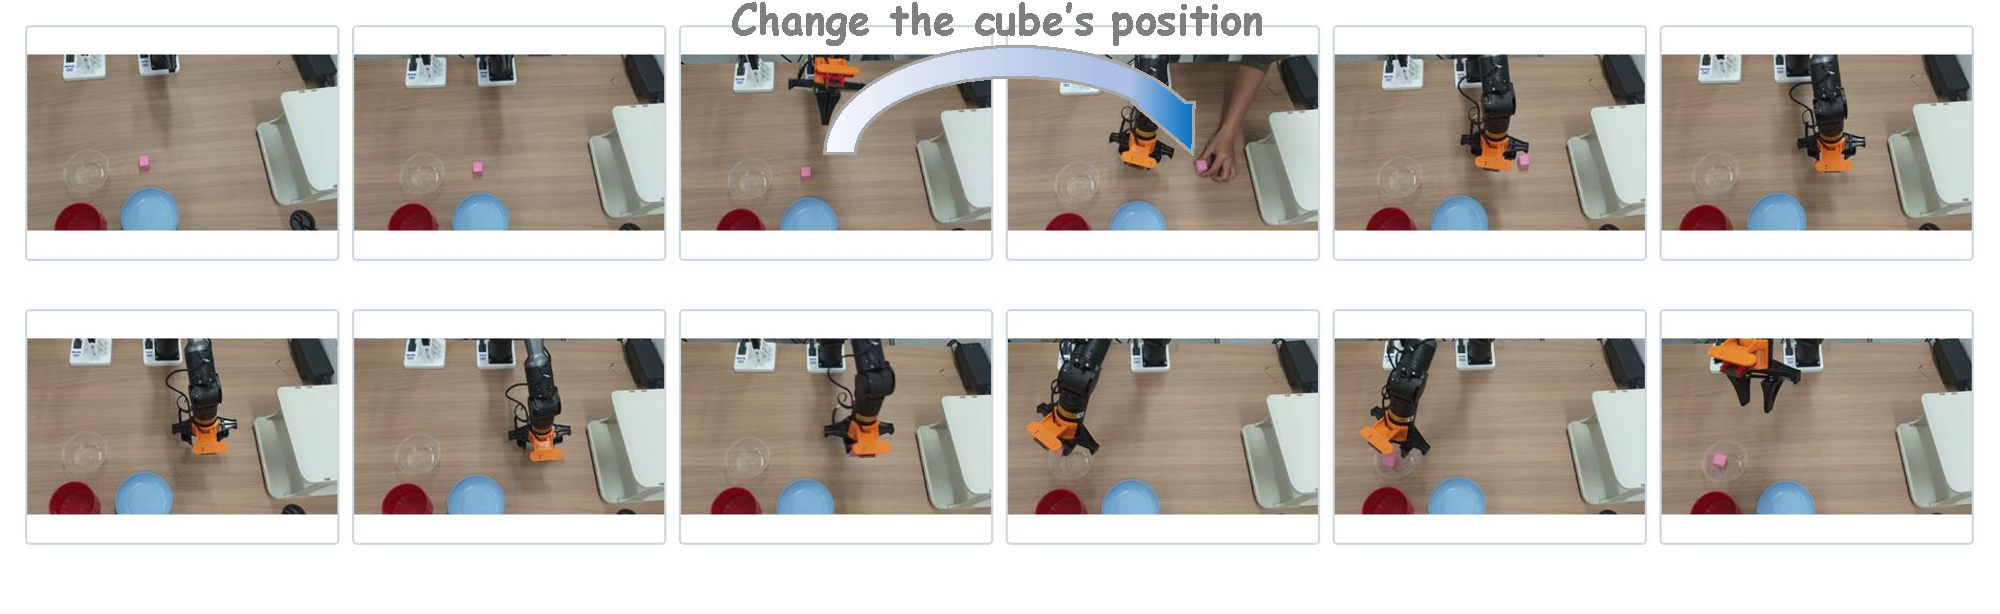
\includegraphics[width=0.95\textwidth]{plots/task_white_bowl.pdf}
    \caption{\textbf{Demo: Moving-object grasp.} The robot picks up the cube and places it into the white bowl, while a human manually changes the cube's position during the process.}
    \label{fig:demo_moving_object_grasp}
\end{figure*}

\begin{figure*}[htbp]
    \centering
    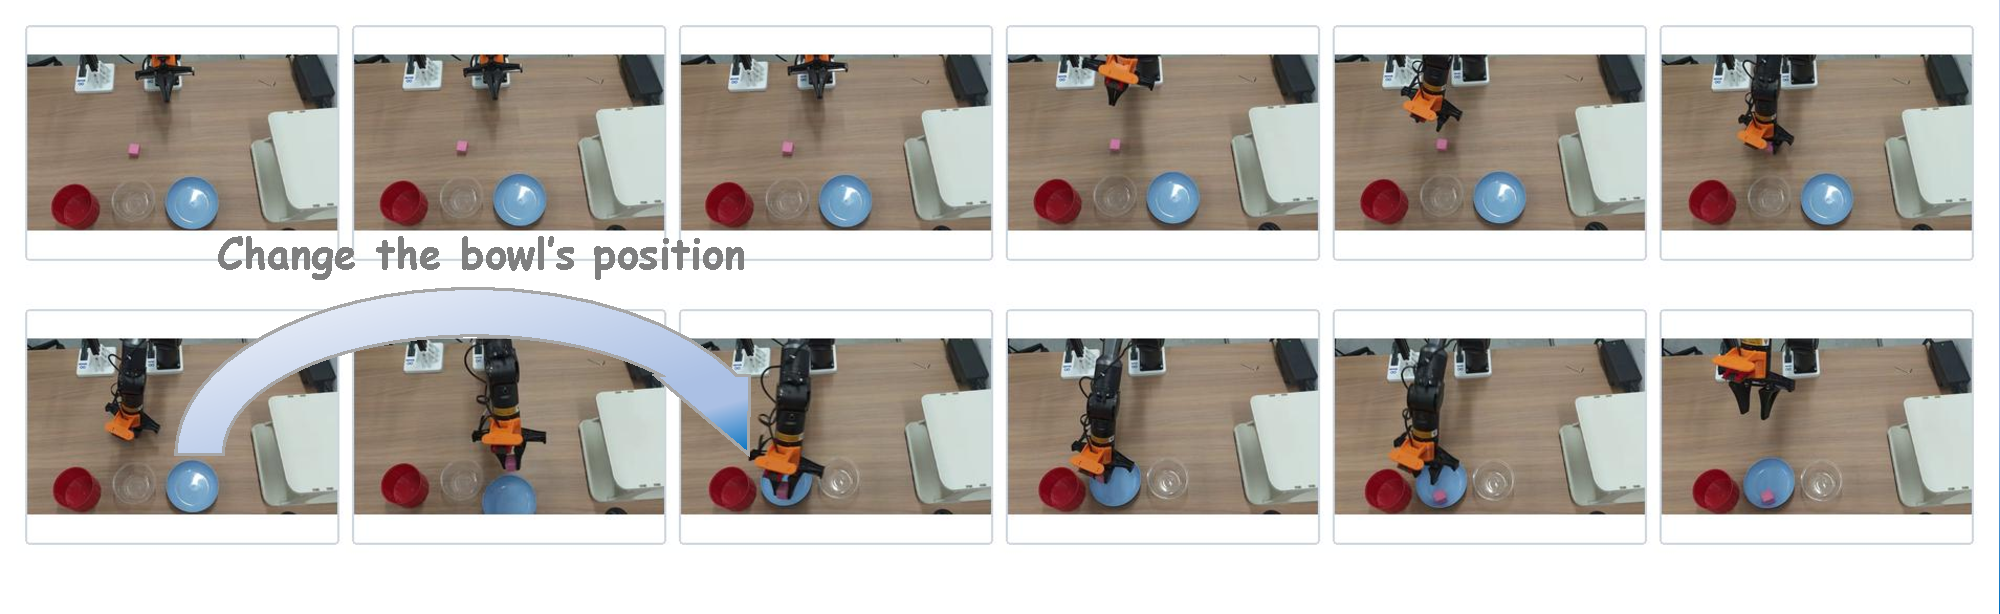
\includegraphics[width=0.95\textwidth]{plots/task_blue_bowl.pdf}
    \caption{\textbf{Demo: Moving-placement target.} The robot picks up the cube and places it into the blue bowl, while a human manually changes the bowl's position during the process.}
    \label{fig:demo_moving_placement_target}
\end{figure*}

\begin{figure*}[htbp]
    \centering
    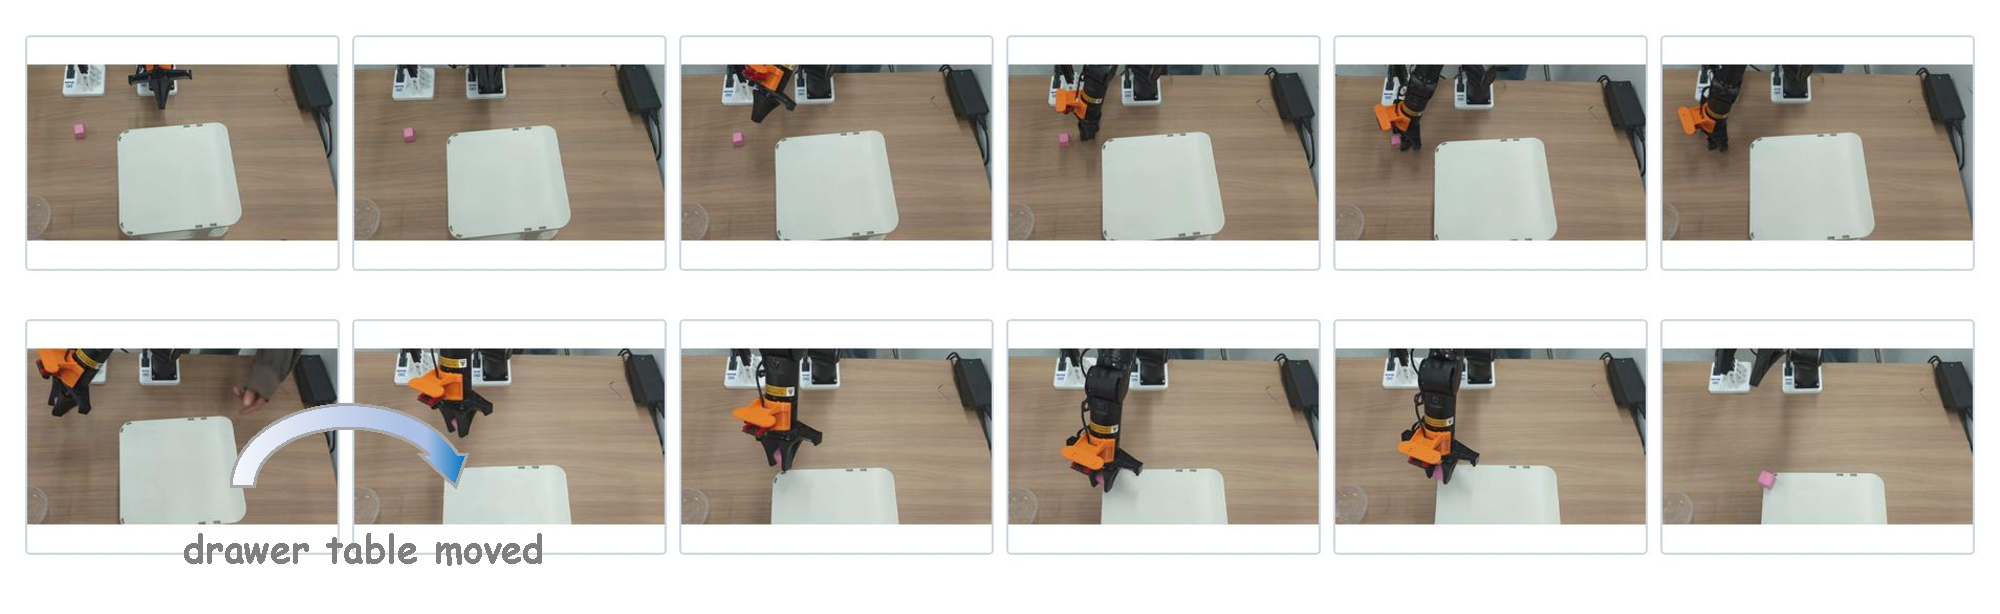
\includegraphics[width=0.95\textwidth]{plots/task_drawer.pdf}
    \caption{\textbf{Demo: Moving-insertion target.} The robot picks up the cube and places it at the upper-left corner of the drawer top, while a human manually changes the drawer's position during the process.}
    \label{fig:demo_moving_insertion_target}
\end{figure*}

